% ***********************************************************
% Dissertation template and document class for
%           The Hong Kong Polytechnic University
% Author  : QING Pei <edwardtoday@gmail.com>
% Adapted from: http://engineering.purdue.edu/~mark/puthesis/
% ***********************************************************


%%% For the electronic copy, use doublespacing,
%   define "\printmode" to get all text black for readability
\documentclass[12pt,lot,lof]{hkputhesis}
\newcommand{\printmode}{}

%%% For early drafts without some of the frontmatter
% Also see the "ifodd" command below to disable more frontmatter
%\documentclass[12pt]{hkputhesis}

%%% The PDF version should be compatible with Acrobat 5.0 or above
%   which make it PDF 1.4
% \pdfoutput=1
\pdfminorversion=4
\pdfobjcompresslevel=0
% \pdfimageresolution=300
% \pdfpkresolution=300
% or you could simply use a package to achieve this
% \RequirePackage{pdf14}

%%%%%%%%%%%%%%%%%%%%%%%%%%%%%%%%%%%%%%%%%%%%%%%%%%%%%%%%%%%%%
%%%% Author & title page info

\title{An hkputhesis sample}

\submitted{July 2012}  % degree conferral date (January, April, June, September, or November)
\copyrightyear{2012}  % year in which the copyright is secured by publication of the dissertation.
\author{QING Pei}
% \adviser{David Zhang}  %replace with the full name of your adviser
% \departmentprefix{Program in}  % defaults to "Department of", but programs need to change this.
% \department{Computing}
\programme{Master of Science in Software Technology}

%%%%%%%%%%%%%%%%%%%%%%%%%%%%%%%%%%%%%%%%%%%%%%%%%%%%%%%%%%%%%
%%%% Tweak float placements
% From: http://mintaka.sdsu.edu/GF/bibliog/latex/floats.html "Controlling LaTeX Floats"
% and based on: http://www.tex.ac.uk/cgi-bin/texfaq2html?label=floats
% LaTeX defaults listed at: http://people.cs.uu.nl/piet/floats/node1.html

% Alter some LaTeX defaults for better treatment of figures:
  % See p.105 of "TeX Unbound" for suggested values.
  % See pp. 199-200 of Lamport's "LaTeX" book for details.
  %   General parameters, for ALL pages:
  \renewcommand{\topfraction}{0.85}	% max fraction of floats at top
  \renewcommand{\bottomfraction}{0.6}	% max fraction of floats at bottom
  %   Parameters for TEXT pages (not float pages):
  \setcounter{topnumber}{2}
  \setcounter{bottomnumber}{2}
  \setcounter{totalnumber}{4}     % 2 may work better
  \setcounter{dbltopnumber}{2}    % for 2-column pages
  \renewcommand{\dbltopfraction}{0.66}	% fit big float above 2-col. text
  \renewcommand{\textfraction}{0.15}	% allow minimal text w. figs
  %   Parameters for FLOAT pages (not text pages):
  \renewcommand{\floatpagefraction}{0.66}	% require fuller float pages
	% N.B.: floatpagefraction MUST be less than topfraction !!
  \renewcommand{\dblfloatpagefraction}{0.66}	% require fuller float pages

% The documentclass already sets parameters to make a high penalty for widows and orphans.

%%%%%%%%%%%%%%%%%%%%%%%%%%%%%%%%%%%%%%%%%%%%%%%%%%%%%%%%%%%%%
%%% Use packages

\usepackage{amsfonts,amsmath}

%%% For figures
\usepackage{graphicx,epstopdf,subfigure}

%%% for comments and listings
\usepackage{verbatim}

%%% For tables
\usepackage{multirow}
\usepackage{multicol}
\usepackage{rotating}

% Longtable lets you have tables that span multiple pages.
\usepackage{longtable}
\usepackage{lscape}
\usepackage[tableposition=top]{caption}
\captionsetup[table]{labelsep=period}  % Change colon in "Table ##:" to "."

% Booktabs produces far nicer tables than the standard LaTeX tables.
%   see: http://en.wikibooks.org/wiki/LaTeX/Tables
\usepackage{booktabs}

%set parameters for longtable:
% default caption width is 4in for longtable, but wider for normal tables
\setlength{\LTcapwidth}{\textwidth}

%%% Date formatting
\usepackage{datetime}

%%% Set fonts
% defines Adobe Times Roman (or equivalent) as default text font
\usepackage{mathptmx}

%%% Set line spacing
\usepackage{setspace}
\onehalfspacing

%%% Turn off indentation globally
\usepackage{parskip}
\setlength{\parskip}{18pt} % to simulate a blank line between paragraphs

%%% Page number at bottom right
\usepackage{fancyhdr}
\fancyhf{} % clear all header and footers
\renewcommand{\headrulewidth}{0pt} % remove the header rule
\rfoot{\fancyplain{\minsize\thepage\hspace{1.8em}}{\minsize\thepage\hspace{1.8em}}}
\pagestyle{fancyplain}

%%% Create hyperlinks for cross-references in the document.
\usepackage{hyperref}
\hypersetup{bookmarksnumbered}
% copy the already-set title and author to use in the pdf properties
\makeatletter
\hypersetup{pdftitle=\@title,pdfauthor=\@author,pdfcreator=\@author}
\makeatother

%%% Setting the margins
\usepackage[top=1in, left=1.8in, bottom=1.4in, right=1.1in]{geometry}

%%% Change chapter heading format (with text shadow)
\usepackage{shadowtext}
\shadowoffsetx{1pt}
\shadowoffsety{.7pt}
\usepackage{titlesec}
\makeatletter
\renewcommand{\@makechapterhead}[1]{%
\vspace*{-6pt}{\setlength{\parindent}{0pt} \raggedright \normalfont
\bfseries\chaptersize \shadowtext{\chaptertitlename\ \thechapter \quad\ #1
}}\vspace*{22pt}}
\makeatother

% change fontsize for section/subsection/subsubsection headings
\titleformat{\section}{\normalfont\sectionsize}{\thesection}{1em}{}
\titleformat{\subsection}{\normalfont\subsectionsize}{\thesubsection}{1em}{}
\titleformat{\subsubsection}{\normalfont\subsubsectionsize}{\thesubsection}{1em}{}

% Change spacing for headings. Please ignore the actual numbers.
% They are tweaked by comparing PDF outputs to the Word template. --!
\titlespacing*{\section}{0pt}{-12pt}{6pt}
\titlespacing*{\subsection}{0pt}{-14pt}{6pt}
\titlespacing*{\subsubsection}{0pt}{-16pt}{6pt}

%%% Change heading format of References
\renewcommand*{\bibname}{References}
\makeatletter
\renewenvironment{thebibliography}[1]{
\clearpage
\ifdefined\phantomsection
\phantomsection
\else
\fi
\addcontentsline{toc}{chapter}{\bibname}
\vspace*{-12pt}
\begin{doublespace}
  {\subsectionsize\bfseries \bibname}
\end{doublespace}
\vspace*{6pt}
\onehalfspacing
\@mkboth{\MakeUppercase\bibname}{\MakeUppercase\bibname}%
\list{\@biblabel{\@arabic\c@enumiv}}{
  \settowidth\labelwidth{\@biblabel{#1}}%
  \leftmargin\labelwidth
  \advance\leftmargin\labelsep
  \@openbib@code
  \usecounter{enumiv}%
  \let\p@enumiv\@empty
  \renewcommand\theenumiv{\@arabic\c@enumiv}}%
\sloppy
\clubpenalty4000
\@clubpenalty \clubpenalty
\widowpenalty4000%
\sfcode`\.\@m}{
  \def\@noitemerr
  {\@latex@warning{Empty `thebibliography' environment}}%
  \endlist}
 \makeatother

%%% Set heading format for Appendix
\usepackage{appendix}
\usepackage{appendix}
\makeatletter
\newcommand\appendix@chapter[1]{
	\refstepcounter{chapter}
	\orig@chapter*{
		\vspace*{-72pt}
		\subsectionsize\bfseries Appendix \@Alph\c@chapter: #1
		\vspace*{-36pt}
	}
	\addcontentsline{toc}{chapter}{Appendix \@Alph\c@chapter: #1}
}
\let\orig@chapter\chapter
\g@addto@macro\appendix{\let\chapter\appendix@chapter}
\makeatother


%%% Set Table of Contents format
\renewcommand\contentsname{Table of Contents}
\usepackage[subfigure]{tocloft}
\renewcommand{\cftbeforechapskip}{0pt}
\renewcommand{\cftbeforetoctitleskip}{6pt}
\renewcommand{\cftaftertoctitleskip}{12pt}
% Set ToC heading size the same as that of Abstract
\renewcommand\cfttoctitlefont{\subsectionsize\bfseries}
\renewcommand\cftchapfont{\tocchapsize\bfseries}
\renewcommand\cftchappresnum{Chapter } % prefix "Chapter " to chapter number in ToC
\cftsetindents{chapter}{0em}{5em}      % set amount of indenting
\makeatletter \renewcommand{\@dotsep}{1} \makeatother
\renewcommand{\cftchapdotsep}{\cftdotsep}

\renewcommand{\cftbeforeloftitleskip}{6pt}
\renewcommand{\cftafterloftitleskip}{18pt}
\renewcommand\cftloftitlefont{\subsectionsize\bfseries}
\renewcommand\cftfigpresnum{Figure }  % prefix "Figure " to entries in LoF
\cftsetindents{figure}{0em}{5em}      % set amount of indenting

\renewcommand{\cftbeforelottitleskip}{6pt}
\renewcommand{\cftafterlottitleskip}{18pt}
\renewcommand\cftlottitlefont{\subsectionsize\bfseries}
\renewcommand\cfttabpresnum{Table }	 % prefix "Table " to entries in LoT
\cftsetindents{table}{0em}{5em}      % set amount of indenting


%%%%%%%%%%%%%%%%%%%%%%%%%%%%%%%%%%%%%%%%%%%%%%%%%%%%%%%%%%%%%
%%% Printed vs. online formatting

\ifdefined\printmode
% url package understands urls (with proper line-breaks) without hyperlinking them
\usepackage{url}
% turn off code highlighting
\usepackage{listings}
\lstset{language=Matlab,
   keywords={break,case,catch,continue,else,elseif,end,for,function,
      global,if,otherwise,persistent,return,switch,try,while},
   basicstyle=\ttfamily,
   keywordstyle=\bfseries\color{black},
   commentstyle=\color{black},
   stringstyle=\color{black},
   numbers=left,
   numberstyle=\tiny\color{black},
   stepnumber=1,
   numbersep=10pt,
   backgroundcolor=\color{white},
   tabsize=4,
   showspaces=false,
   showstringspaces=false}
\else
% Online copy
% turn on code highlighting
\usepackage{color}
\usepackage{listings}
\definecolor{dkgreen}{rgb}{0,0.6,0}
\definecolor{gray}{rgb}{0.5,0.5,0.5}
\lstset{language=Matlab,
   keywords={break,case,catch,continue,else,elseif,end,for,function,
      global,if,otherwise,persistent,return,switch,try,while},
   basicstyle=\ttfamily,
   keywordstyle=\color{blue},
   commentstyle=\color{gray},
   stringstyle=\color{dkgreen},
   numbers=left,
   numberstyle=\tiny\color{red},
   stepnumber=1,
   numbersep=10pt,
   backgroundcolor=\color{white},
   tabsize=4,
   showspaces=false,
   showstringspaces=false}

% make the page number rather than the text be the link for ToC entries
%\hypersetup{linktocpage}

\fi % print or online formatting


%%%%%%%%%%%%%%%%%%%%%%%%%%%%%%%%%%%%%%%%%%%%%%%%%%%%%%%%%%%%%
%%%% Define commands

% Define any custom commands that you want to use.
% For example, highlight notes for future edits to the thesis
%\newcommand{\todo}[1]{\textbf{\emph{TODO:}#1}}


% create an environment that will indent text
% see: http://latex.computersci.org/Reference/ListEnvironments
% 	\raggedright makes them left aligned instead of justified
\newenvironment{indenttext}{
\begin{list}{}{ \itemsep 0in \itemindent 0in
\labelsep 0in \labelwidth 0in
\listparindent 0in
\topsep 0in \partopsep 0in \parskip 0in \parsep 0in
\leftmargin 1em \rightmargin 0in
\raggedright
}
\item
}
{\end{list}}

% another environment that's an indented list, with no spaces
% between items -- if we want multiple items/lines. Useful in
% tables. Use \item inside the environment.
% \raggedright makes them left aligned instead of justified
\newenvironment{indentlist}{
\begin{list}{}{ \itemsep 0in \itemindent 0in
\labelsep 0in \labelwidth 0in
\listparindent 0in
\topsep 0in \partopsep 0in \parskip 0in \parsep 0in
\leftmargin 1em \rightmargin 0in
\raggedright
}

}
{\end{list}}

%
%  mydefs.tex  2007-03-19  Mark Senn  http://www.ecn.purdue.edu/~mark
%
%  Command definitions that can be used in all documents that have
%      %
%  mydefs.tex  2007-03-19  Mark Senn  http://www.ecn.purdue.edu/~mark
%
%  Command definitions that can be used in all documents that have
%      %
%  mydefs.tex  2007-03-19  Mark Senn  http://www.ecn.purdue.edu/~mark
%
%  Command definitions that can be used in all documents that have
%      \input{mydefs}
%

% CHANGE NEXT 3 LINES?
% Define \be and \ee to start and end the equation environment.
\newcommand{\be}{\begin{equation}}
\newcommand{\ee}{\end{equation}}

% CHANGE NEXT 12 LINES?
% Define \Repeat so, for example,
%     \Repeat{whatever}{10}
% is the same as typing whatever 10 times.
\newcount{\myi}
\newcommand{\Repeat}[2]{%
    \myi=0
    \loop
        \ifnum\myi<#2
        #1
        \advance\myi by 1
    \repeat
}

% CHANGE NEXT 3 LINES?
% Make "\Sum ab" or "\Sum{a}{b}" do "\sum_{a}^{b}".
% This can only be used when in math mode.
\newcommand\Sum[2]{\sum_{#1}^{#2}}

% CHANGE NEXT 4 LINES?
% Make "\xn" do "$x_n$".
% Because this definition contains the "$" to go into math mode
% this definition must be used when not in math mode.
\newcommand{\xn}{$x_n$}

% CHANGE NEXT 5 LINES?
% Since \xn is already defined we must use \renewcommand to redefine it.
% Normally you would not have the above definition for \xn in this file
% if you were just going to override it later.
% The \ensuremath goes into math mode if not already in math mode.
\renewcommand{\xn}{\ensuremath{x_n}}


%

% CHANGE NEXT 3 LINES?
% Define \be and \ee to start and end the equation environment.
\newcommand{\be}{\begin{equation}}
\newcommand{\ee}{\end{equation}}

% CHANGE NEXT 12 LINES?
% Define \Repeat so, for example,
%     \Repeat{whatever}{10}
% is the same as typing whatever 10 times.
\newcount{\myi}
\newcommand{\Repeat}[2]{%
    \myi=0
    \loop
        \ifnum\myi<#2
        #1
        \advance\myi by 1
    \repeat
}

% CHANGE NEXT 3 LINES?
% Make "\Sum ab" or "\Sum{a}{b}" do "\sum_{a}^{b}".
% This can only be used when in math mode.
\newcommand\Sum[2]{\sum_{#1}^{#2}}

% CHANGE NEXT 4 LINES?
% Make "\xn" do "$x_n$".
% Because this definition contains the "$" to go into math mode
% this definition must be used when not in math mode.
\newcommand{\xn}{$x_n$}

% CHANGE NEXT 5 LINES?
% Since \xn is already defined we must use \renewcommand to redefine it.
% Normally you would not have the above definition for \xn in this file
% if you were just going to override it later.
% The \ensuremath goes into math mode if not already in math mode.
\renewcommand{\xn}{\ensuremath{x_n}}


%

% CHANGE NEXT 3 LINES?
% Define \be and \ee to start and end the equation environment.
\newcommand{\be}{\begin{equation}}
\newcommand{\ee}{\end{equation}}

% CHANGE NEXT 12 LINES?
% Define \Repeat so, for example,
%     \Repeat{whatever}{10}
% is the same as typing whatever 10 times.
\newcount{\myi}
\newcommand{\Repeat}[2]{%
    \myi=0
    \loop
        \ifnum\myi<#2
        #1
        \advance\myi by 1
    \repeat
}

% CHANGE NEXT 3 LINES?
% Make "\Sum ab" or "\Sum{a}{b}" do "\sum_{a}^{b}".
% This can only be used when in math mode.
\newcommand\Sum[2]{\sum_{#1}^{#2}}

% CHANGE NEXT 4 LINES?
% Make "\xn" do "$x_n$".
% Because this definition contains the "$" to go into math mode
% this definition must be used when not in math mode.
\newcommand{\xn}{$x_n$}

% CHANGE NEXT 5 LINES?
% Since \xn is already defined we must use \renewcommand to redefine it.
% Normally you would not have the above definition for \xn in this file
% if you were just going to override it later.
% The \ensuremath goes into math mode if not already in math mode.
\renewcommand{\xn}{\ensuremath{x_n}}



%%%%%%%%%%%%%%%%%%%%%%%%%%%%%%%%%%%%%%%%%%%%%%%%%%%%%%%%%%%%%
%%%% Front-matter

% For early drafts, you may want to disable some of the frontmatter.
% Simply change this to "\ifodd 1" to do so.
\ifodd 0
% front-matter disabled while writing chapters
\renewcommand{\maketitlepage}{}
\renewcommand*{\makeauthorshipstatement}{}
\renewcommand*{\makeabstract}{}

% you can just skip the \acknowledgements and \dedication commands
% to leave out these sections.

\else

\abstract{
% Import the abstract file.
%!TEX root = thesis.tex

This is the abstract.

}

\acknowledgements{
%I would like to thank...
%!TEX root = thesis.tex

This is the acknowledgments.

}

% \dedication{To my parents.}

\fi  % disable frontmatter


%%%%%%%%%%%%%%%%%%%%%%%%%%%%%%%%%%%%%%%%%%%%%%%%%%%%%%%%%%%%%
%%%% Hide some chapters

%%% If you want to produce a pdf that includes only certain chapters, specify
%   them with includeonly, in addition to including all chapters below.
%\includeonly{ch-intro/chapter-intro}
%%% You can also specify multiple chapters.
%\includeonly{ch-intro/chapter-intro,ch-usage/chapter-usage}
%\includeonly{chap1,chap2,chap3}


%%%%%%%%%%%%%%%%%%%%%%%%%%%%%%%%%%%%%%%%%%%%%%%%%%%%%%%%%%%%%
%%%% Notes:

% Footnotes should be placed after punctuation.\footnote{place here.}
% Generally, place citations before the period~\cite{anotherauthor}.
% The proper usage for i.e., and e.g., include commas ``(e.g., option A, option B)''

%%%%%%%%%%%%%%%%%%%%%%%%%%%%%%%%%%%%%%%%%%%%%%%%%%%%%%%%%%%%%
%%%% Import chapters
\begin{document}

\makefrontmatter
\pagestyle{fancy}

% If you've disabled frontmatter, you can insert the toc manually
%\tableofcontents\clearpage

% \include lets us split up the document (and each include starts a new page):
%
%  revised  introduction.tex  2011-09-02  Mark Senn  http://engineering.purdue.edu/~mark
%  created  introduction.tex  2002-06-03  Mark Senn  http://engineering.purdue.edu/~mark
%
%  This is the introduction chapter for a simple, example thesis.
%


\chapter{Introduction}

This is the introduction.
The first paragraph after a heading is not indented.

This is a sentence.
This is a sentence.
This is a sentence.
This is a sentence.
This is a sentence.


\section{Section Heading}

This is a sentence.
This is a sentence.
This is a sentence.
This is a sentence.
This is a sentence.


\subsection{Subsection heading}

This is a sentence.
This is a sentence.
This is a sentence.
This is a sentence.
This is a sentence.


\subsubsection{Subsubsection heading}

This is a sentence.
This is a sentence.
This is a sentence.
This is a sentence.
This is a sentence.

%
%  summary.tex  2007-02-06  Mark Senn  http://www.ecn.purdue.edu/~mark
%

\chapter{Summary}

This is the summary chapter.



% include your .bib file
\bibliographystyle{unsrt}
\bibliography{thesis}

\appendix % all chapters following will be labeled as appendices
%
%  revised  demo-citations.tex  2011-09-02  Mark Senn  http://www.ecn.purdue.edu/~mark
%  created  demo-citations.tex  2007-03-21  Mark Senn  http://www.ecn.purdue.edu/~mark
%


\chapter{Demonstrate Citations}

I typed

\begin{verbatim}
    For \LaTeX\ answers I refer to
    % note to self: {\em \LaTeX: A Document Preparation System\/}
    \cite{Lamport:1994}
    and then to
    % note to self: {\em The \LaTeX\ Companion\/}
    \cite{Goossens:1994}
    or
    % note to self: {\em A Guide to LaTeX\/} (1999)
    \cite{Kopka:1999}.
    % note to self: {\em A Guide to LaTeX\/} (1999)
    \cite{Kopka:1999}
    is an updated edition of the 1995 edition
    \cite{Kopka:1995}.
\end{verbatim}

to get

\begin{quotation}
    For \LaTeX\ answers I refer to
    % note to self: {\em \LaTeX: A Document Preparation System\/}
    \cite{Lamport:1994}
    and then to
    % note to self: {\em The \LaTeX\ Companion\/}
    \cite{Goossens:1994}
    or
    % note to self: {\em A Guide to LaTeX\/} (1999)
    \cite{Kopka:1999}.
    % note to self: {\em A Guide to LaTeX\/} (1999)
    \cite{Kopka:1999}
    is an updated edition of the 1995 edition
    \cite{Kopka:1995}.
\end{quotation}

%
%  demo-figures.tex  2009-10-30  Mark Senn  http://engineering.purdue.edu/~mark
%
%  Demonstrate how to do figures.
%

\chapter{Demonstrate Figures}

The
\verb+h+
specifier used in all the examples below
tells \LaTeX\ to put the figure
``here''
instead of trying
to find a good spot
at the top or bottom of a page.
Specifiers can be combined, for example,
``\verb+\begin{figure}[htbp!]+''.

The complete list of specifiers:

\begin{center}
    \renewcommand{\baselinestretch}{1}\normalsize
    \begin{tabular}{ll}
        \bf Specifier& \bf Description\cr
        \tt b& bottom of page\cr
        \tt h& here on page\cr
        \tt p& on separate page of figures\cr
        \tt t& top of page\cr
        \tt !& try hard to put figure as early as possible\cr
    \end{tabular}
\end{center}

Label ``fi:not-centered'' is ``\ref{fi:not-centered}''.
Label ``sf:four-parts-c'' is ``\ref{sf:four-parts-c}''.

\Repeat{This is the first paragraph.}{5}

\begin{figure}[h]
  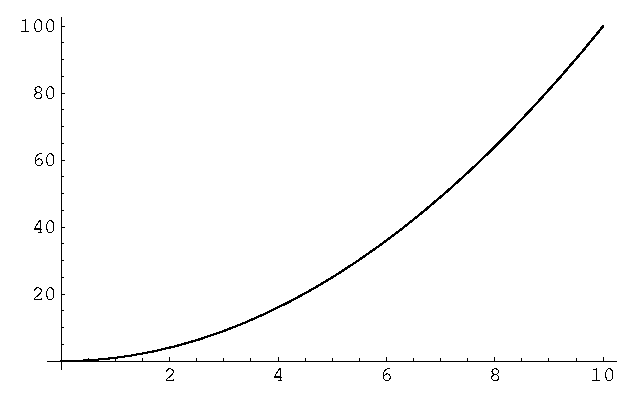
\includegraphics{plot.eps}
  \caption{%
    By default figures are not centered.
    This is a long caption to demonstrate that captions are single spaced.
  }
  \label{fi:not-centered}
\end{figure}

\Repeat{This is the second paragraph.}{10}

\begin{figure}[h]
  \centering
  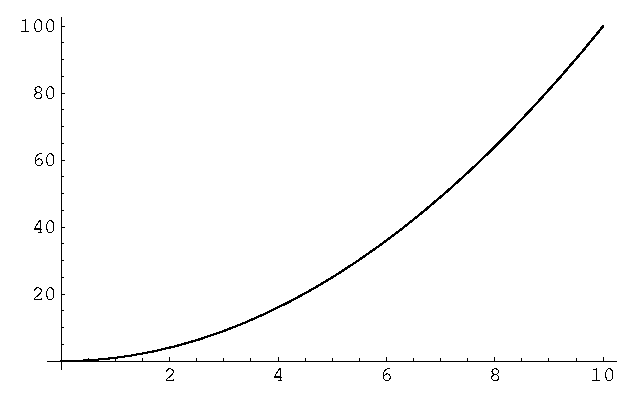
\includegraphics{plot.eps}
  \caption{Use {\tt \char'134centering\/} to center figures.}
  \label{fi:centered}
\end{figure}

\Repeat{This is the third paragraph.}{15}

\begin{figure}[h]
  \centering
  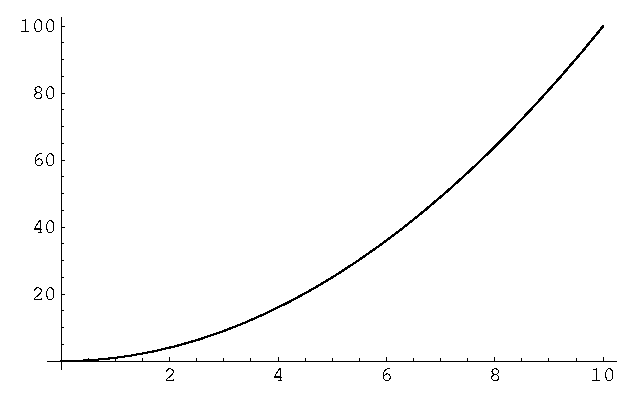
\includegraphics{plot.eps}
  \caption{This is another figuure.}
  \label{fi:another}
\end{figure}

\Repeat{This is the fourth paragraph.}{10}

\begin{figure}[h]
  \centering
  \subfigure[First subcaption.]{\label{sf:two-parts-a}  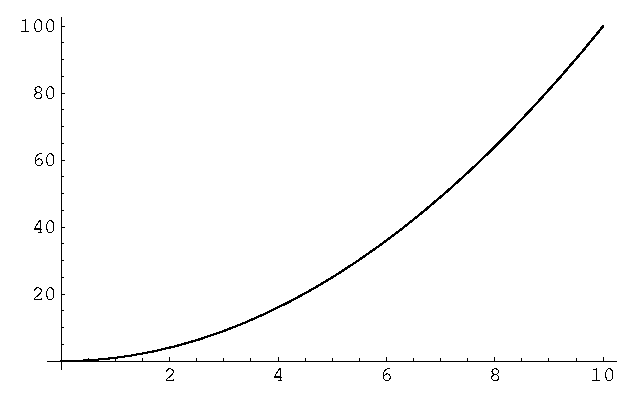
\includegraphics[width=0.3\textwidth]{plot.eps}}%
  \hskip 0.5truein
  \subfigure[Second subcaption.]{\label{sf:two-parts-b}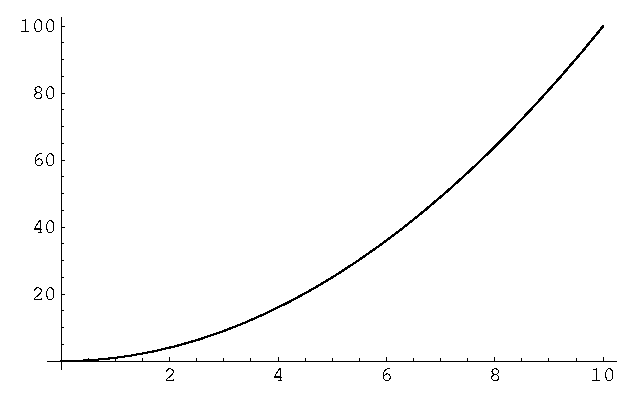
\includegraphics[width=0.3\textwidth]{plot.eps}}
  \caption{This figure has two parts.}
  \label{fi:two-parts}
\end{figure}

\Repeat{This is the fifth paragraph.}{10}

\begin{figure}[h]
  \centering
  \subfigure[First subcaption.]{\label{sf:four-parts-a}  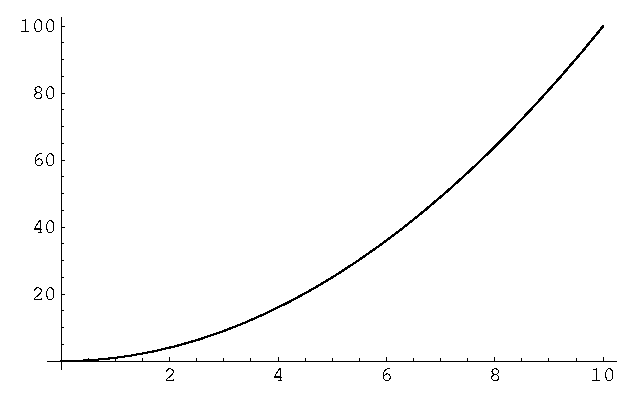
\includegraphics[width=0.3\textwidth]{plot.eps}}%
  \hskip 0.5truein
  \subfigure[Second subcaption.]{\label{sf:four-parts-b}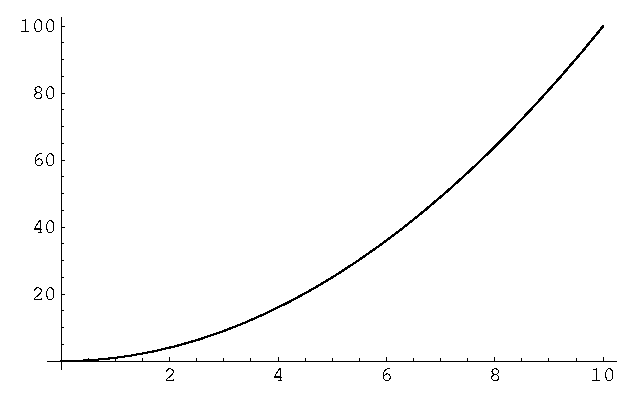
\includegraphics[width=0.3\textwidth]{plot.eps}}
  \subfigure[Third subcaption.]{\label{sf:four-parts-c}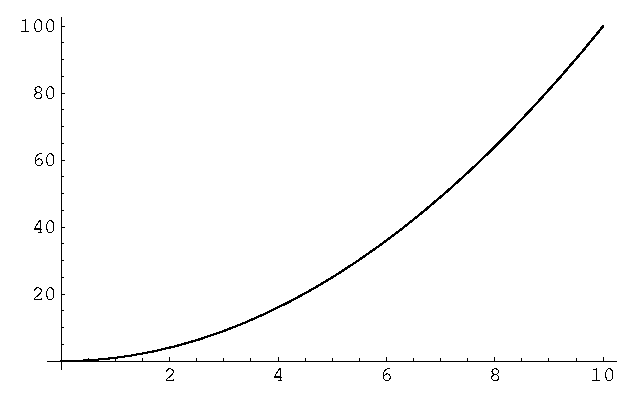
\includegraphics[width=0.3\textwidth]{plot.eps}}%
  \hskip 0.5truein
  \subfigure[Fourth subcaption.]{\label{sf:four-parts-d}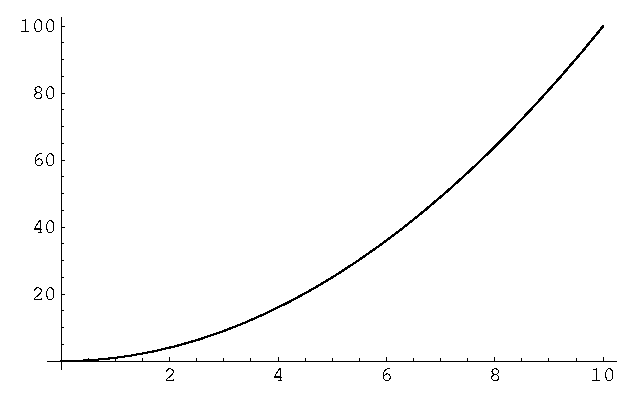
\includegraphics[width=0.3\textwidth]{plot.eps}}
  \caption{This figure has four parts.}
  \label{fi:four-parts}
\end{figure}

\Repeat{This is the sixth paragraph.}{10}

%
%  THIS FILE DOES SOME UNUSUAL THINGS TO MAKE
%  IT EASIER TO DO DEMONSTRATIONS.  IT SHOULD
%  NOT BE USED AS AN EXAMPLE OF HOW TO PREPARE
%  A FILE.  SEE THE OUTPUT OF THIS FOR LATEX
%  INPUT AND OUTPUT EXAMPLES.
%




%
%  demo-mathematics.tex  2008-12-09  Mark Senn  http://engineering.purdue.edu/~mark
%

\chapter{Demonstrate Mathematics}
    % You don't normally need this.
    \mbox{}

    \begin{verbatim}
% From _More Math Into LaTeX_, 4th Edition, page 152:
%     TeX uses $$ to open and close a displayed math environment.
%     In LaTeX, this may occassionally cause problems.  Don't do it.
\[
    E = mc^2
\]
    \end{verbatim}
% From _More Math Into LaTeX_, 4th Edition, page 152:
%     TeX uses $$ to open and close a displayed math environment.
%     In LaTeX, this may occassionally cause problems.  Don't do it.
\[
    E = mc^2
\]
    \vskip\baselineskip
    \hrule
    \vskip0.5\baselineskip
    \filbreak

    \begin{verbatim}
\begin{equation}
    E = mc^2
\end{equation}
    \end{verbatim}
\begin{equation}
    E = mc^2
\end{equation}
    \vskip\baselineskip
    \hrule
    \vskip0.5\baselineskip
    \filbreak

    \begin{verbatim}
% Mydefs.tex defines \be to be \begin{equation} and
% \ee to be \end{equation}.
\be
    E = mc^2
\ee
    \end{verbatim}
% Mydefs.tex defines \be to be \begin{equation} and
% \ee to be \end{equation}.
\be
    E = mc^2
\ee
    \vskip\baselineskip
    \hrule
    \vskip0.5\baselineskip
    \filbreak

    \begin{verbatim}
\be
    x = -\frac{b}{2a} \pm \frac{\sqrt{b^2 - 4ac}}{2a}
\ee
    \end{verbatim}
\be
    x = -\frac{b}{2a} \pm \frac{\sqrt{b^2 - 4ac}}{2a}
\ee
    \vskip\baselineskip
    \hrule
    \vskip0.5\baselineskip
    \filbreak

    \begin{verbatim}
% requires \usepackage{amsmath}; use align* for no equation number
\begin{align}
    a = {}& b + c\\
    x = {}& y + z
\end{align}
    \end{verbatim}
% requires \usepackage{amsmath}; use align* for no equation number
\begin{align}
    a = {}& b + c\\
    x = {}& y + z
\end{align}
    \vskip\baselineskip
    \hrule
    \vskip0.5\baselineskip
    \filbreak

    \begin{verbatim}
\[
    Z = \left(
        \begin{array}{cc}
            a& b\\
            c& d
        \end{array}
    \right)
\]
    \end{verbatim}
\[
    Z = \left(
        \begin{array}{cc}
            a& b\\
            c& d
        \end{array}
    \right)
\]
    \vskip\baselineskip
    \hrule
    \vskip0.5\baselineskip
    \filbreak

    \begin{verbatim}
\begin{equation}
    \begin{split}
        a = {}& b + c\\
            {}& + d + e
    \end{split}
\end{equation}
    \end{verbatim}
\begin{equation}
    \begin{split}
        a = {}& b + c\\
            {}& + d + e
    \end{split}
\end{equation}
    \vskip\baselineskip
    \hrule
    \vskip0.5\baselineskip
    \filbreak

    \begin{verbatim}
\be
    (\cos x)^2 + (\sin x)^2 = 1
\ee
    \end{verbatim}
\be
    (\cos x)^2 + (\sin x)^2 = 1
\ee
    \vskip\baselineskip
    \hrule
    \vskip0.5\baselineskip
    \filbreak

    \begin{verbatim}
If $X = \cos x$ and $Y = \sin x$ then $X^2 + Y^2 = 1$.
    \end{verbatim}
If $X = \cos x$ and $Y = \sin x$ then $X^2 + Y^2 = 1$.
    \vskip\baselineskip
    \hrule
    \vskip0.5\baselineskip
    \filbreak

%
%  demo-multicols.tex  2007-03-19  Mark Senn  http://www.ecn.purdue.edu/~mark
%
%  Demonstrate multicols.
%
%  The multicols package must be loaded for this to work.
%  To load the multicols package put
%      \usepackage{multicols}
%  between the "\documentclass" and "\begin{document}" commands.
%

\chapter{Demonstrate Multicols}

% Put this amount of space between the columns.
\setlength{\columnsep}{0.5truein}

% Separate the columns with a vertical rule this wide.
\setlength{\columnseprule}{0.4pt}

\Repeat{This is one column.}{25}

\begin{multicols}{2}
\Repeat{This is two columns.}{25}
\end{multicols}

\begin{multicols}{3}
\Repeat{This is three columns.}{25}
\end{multicols}

\begin{multicols}{4}
\Repeat{This is four columns.}{25}
\end{multicols}

\begin{multicols}{5}
\Repeat{This is five columns.}{25}
\end{multicols}

%
%  demo-tables.tex  2009-09-29  Mark Senn  http://engineering.purdue.edu/~mark
%
%  Demonstrate how to do tables.
%

\chapter{Demonstrate Tables}

\begin{tabular}{ll}
    \bf Label& \bf Number\\
    ta:text-only& \ref{ta:text-only}\\
    ta:fruit&     \ref{ta:fruit}
\end{tabular}

\newlength{\ta}
\newlength{\tb}
\newlength{\tc}

\settowidth{\ta}{\vbox{\hbox{Money}\hbox{Market}}}
\settowidth{\tb}{\vbox{\hbox{Stocks}\hbox{and}\hbox{Bonds}}}
\settowidth{\tc}{\vbox{\hbox{Money}\hbox{Market}\hbox{and}\hbox{Stocks}}}

%{\renewcommand{\baselinestretch}{1}
%  \begin{table}
%    \caption{%
%      \hfil Allocation of the IRA and Keogh Wealth\hfil\break
%      \mbox{}\hfil for Investors With or Without Brokerage Accounts\hfil
%    }
%    \label{tab:ira}
%    \begin{center}
%      \begin{tabular}%
%        {%
%          |%
%          c%
%          |%
%          >{\centering\hspace{0pt}}m{\the\ta}%  Money Market
%          |%
%          c%                                    Stocks 
%          |%
%          c%                                    Bonds
%          |%
%          c%                                    Diversified
%          |%
%          >{\centering\hspace{0pt}}m{\the\tb}%  Stocks and Bonds
%          |%
%          >{\centering\hspace{0pt}}m{\the\tc}%  Money Market and Stocks
%          |%
%          c%                                    Others
%          |%
%        }
%        \hline
%        IMP&
%          Money Market&
%          Stocks&
%          Bonds&
%          Diversified&
%          Stocks and Bonds&
%          Money Market and Stocks&
%          Others\tabularnewline
%        \hline
%        1& 14.19\%& 57.71\%& 12.21\%& 4.50\%& 7.36\%& 3.04\%& 0.99\%\tabularnewline \hline
%        2& 14.08\%& 58.18\%& 12.32\%& 4.44\%& 7.30\%& 2.80\%& 0.88\%\tabularnewline \hline
%        3 &14.26\%& 58.09\%& 12.27\%& 4.50\%& 7.19\%& 2.75\%& 0.94\%\tabularnewline \hline
%        4 &13.94\%& 58.11\%& 12.14\%& 4.78\%& 7.35\%& 2.68\%& 0.99\%\tabularnewline \hline
%        5 &13.92\%& 58.13\%& 11.93\%& 4.56\%& 7.60\%& 2.98\%& 0.88\%\tabularnewline \hline
%      \end{tabular}
%    \end{center}
%    This table presents the allocations of the wealth in the IRA
%    and Keogh accounts in various asset classes.
%    Results from each set of imputed data are presented here.
%    The first column lists the number of the imputations,
%    and rest of the columns lists various allocations.
%    Entrees under each asset class show the percentage of investors
%    who have most of their IRA
%    and Keogh wealth invested in that particular asset class.
%    The asset class Diversified
%    includes stocks,
%    bonds,
%    and money market investments.
%    The asset class Others
%    include investments in various life insurance products,
%    annuities,
%    real estate, etc.
%    \medskip
%    \footnotesize SOURCE: Survey of Consumer Finances,
%    2001,
%    Federal Reserve Board,
%    USA.\par
%  \end{table}
%}

\begin{table}
    This table contains only text.
    Let's cite Lamport's book here: \cite{Lamport:1994}.
    \caption{%
        This is the caption.
        Let's cite Lamport's book again here: \cite{Lamport:1994}.%
    }
    \label{ta:text-only}
\end{table}

\begin{table}
    % \halign{...} is more flexible than \begin{table}...\end{table}.
    \hbox to \textwidth{%
         \hfill
        \vbox{\halign{
            \strut #&            % 0. \strut
            #\hfil\qquad&        % 1. left
            \hfil #\hfil\qquad&  % 2. center
            \hfil #\cr           % 3. right
            %
            & apple& banana& cherry\cite{Lamport:1994}\cr
            & aardvark& boa constrictor& coyote\cr
        }}
        \hfill
    }
    \caption[short caption for table of contents]{%
        This is a really long and boring caption.
        It goes on and on as if it thinks what it says is important.
        Here is some more of it.
        The citation for ``Lamport::1994'' is ``\cite{Lamport:1994}''.%
    }
    \label{ta:fruit}
\end{table}

% This is loosely based on page 106 of _A Guide to LaTeX_, third edition,
% by Helmut Kopka and Patrick W. Daly.
%\begin{longtable}{|l|l|}
%  \caption{2.2 ``State'' Abbreviations}\\
%  \hline
%  ``State''& Abbreviation\\
%  \hline \endfirsthead
%  \caption[]{\emph{continued}}\\
%  \hline
%  ``State''& Abbreviation\\
%  \hline \endhead
%  \hline
%  \multicolumn{2}{r}{\emph{continued on next page}}
%  \endfoot
%  \hline\endlastfoot
%  Alabama& AL\\
%  Alaska& AK\\
%  American Samoa& AS\\
%  Arizona& AZ\\
%  Arkansas& AR\\
%  Armed Forces Europe& AE\\
%  Armed Forces Pacific& AP\\
%  Armed Forces the Americas& AA\\
%  California& CA\\
%  Colorado& CO\\
%  Connecticut& CT\\
%  Delaware& DE\\
%  District of Columbia& DC\\
%  Federated States of Micronesia& FM\\
%  Florida& FL\\
%  Georgia& GA\\
%  Guam& GU\\
%  Hawaii& HI\\
%  Idaho& ID\\
%  Illinois& IL\\
%  Indiana& IN\\
%  Iowa& IA\\
%  Kansas& KS\\
%  Kentucky& KY\\
%  Louisiana& LA\\
%  Maine& ME\\
%  Marshall Islands& MH\\
%  Maryland& MD\\
%  Massachusetts& MA\\
%  Michigan& MI\\
%  Mississippi& MS\\
%  Missouri& MO\\
%  Montana& MT\\
%  N Minnesota
%  Nebraska& NE\\
%  Nevada& NV\\
%  New Hampshire& NH\\
%  New Jersey& NJ\\
%  New Mexico& NM\\
%  New York& NY\\
%  North Carolina& NC\\
%  North Dakota& ND\\
%  Northern Mariana Islands& MP\\
%  Ohio& OH\\
%  Oklahoma& OK\\
%  Oregon& OR\\
%  Pennsylvania& PA\\
%  Puerto Rico& PR\\
%  Rhode Island& RI\\
%  South Carolina& SC\\
%  South Dakota& SD\\
%  Tennessee& TN\\
%  Texas& TX\\
%  Utah& UT\\
%  Vermont& VT\\
%  Virgin Islands, U.S.& VI\\
%  Virginia& VA\\
%  Washington& WA\\
%  West Virginia& WV\\
%  Wisconsin& WI\\
%  Wyoming& WY\\
%\end{longtable}

\newcommand{\cbackslash}{\char'134}
\newcommand{\copencurly}{\char'173}
\newcommand{\cclosecurly}{\char'175}

\newlength{\twidth}
\newlength{\theight}

\setlength{\twidth}{\textwidth}
\setlength{\theight}{\textheight}

\begin{sidewaystable}
    % The following two lines compensate for what I think is a bug.
    \setlength{\textwidth}{\theight}
    \setlength{\textheight}{\twidth}
    \caption{%
        2.3 sidewaystable mode
        {\tt\cbackslash begin\copencurly table\cclosecurly\/}%
        \ldots
        {\tt\cbackslash end\copencurly table\cclosecurly\/} table%
    }
    \hbox to \textwidth{
        \hfill
        \begin{tabular}{lcr}
            apple& banana& cherry\\
            aardvark& boa constrictor& coyote\\
        \end{tabular}
        \hfill
    }
\end{sidewaystable}

\begin{sidewaystable}
    % The following two lines compensate for what I think is a bug.
    \setlength{\textwidth}{\theight}
    \setlength{\textheight}{\twidth}
    \caption{%
        2.4 sidewaystable mode
        {\tt\cbackslash halign\copencurly ...\cclosecurly\/} table%
    }
    \hbox to \textwidth{%
        \hfill
        \vbox{\halign{
            \strut #&            % 0. \strut
            #\hfil\qquad&        % 1. left
            \hfil #\hfil\qquad&  % 2. center
            \hfil #\cr           % 3. right
            %
            & apple& banana& cherry\cr
            & aardvark& boa constrictor& coyote\cr
        }}
        \hfill
    }
\end{sidewaystable}

\begin{table}
    \begin{tabular}{lcr}
        apple& banana& cherry\\
        aardvark& boa constrictor& coyote\\
        apple& banana& cherry\\
        aardvark& boa constrictor& coyote\\
        apple& banana& cherry\\
        aardvark& boa constrictor& coyote\\
        apple& banana& cherry\\
        aardvark& boa constrictor& coyote\\
        apple& banana& cherry\\
        aardvark& boa constrictor& coyote\\
        apple& banana& cherry\\
        aardvark& boa constrictor& coyote\\
        apple& banana& cherry\\
        aardvark& boa constrictor& coyote\\
        apple& banana& cherry\\
        aardvark& boa constrictor& coyote\\
    \end{tabular}
    \caption{2.5 left hand table}
\end{table}

\begin{table}
    \begin{tabular}{lcr}
        apple& banana& cherry\\
        aardvark& boa constrictor& coyote\\
    \end{tabular}
    \caption{2.6 left hand table}
\end{table}

\begin{sidewaystable}
    % The following two lines compensate for what I think is a bug.
    \setlength{\textwidth}{\theight}
    \setlength{\textheight}{\twidth}
    \caption{%
        2.7 sidewaystable mode
        {\tt\cbackslash begin\copencurly table\cclosecurly\/}%
        \ldots
        {\tt\cbackslash end\copencurly table\cclosecurly\/} table%
    }
    \hbox to \textwidth{%
        \hfill
        \begin{tabular}{lcr}
            apple& banana& cherry\\
            aardvark& boa constrictor& coyote\\
        \end{tabular}
        \hfill
    }
\end{sidewaystable}

%\newlength{\ta}
%\settowidth{\ta}{\vbox{\hbox{Money}\hbox{Market}}}
%\newlength{\tb}
%\settowidth{\tb}{\vbox{\hbox{Stocks}\hbox{and}\hbox{Bonds}}}
%\newlength{\tc}
%\settowidth{\tc}{\vbox{\hbox{Money}\hbox{Market}\hbox{and}\hbox{Stocks}}}
%
%  {\renewcommand{\baselinestretch}{1}
%\begin{table}
%  \caption{\hfil Allocation of the IRA and Keogh Wealth\hfil\break\mbox{}\hfil for Investors With or Without Brokerage Accounts\hfil}
%  \label{tab:ira}
%  \begin{center}
%    \begin{tabular}%
%      {%
%        |%
%        c%
%        |%
%        >{\centering\hspace{0pt}}m{\the\ta}%  Money Market
%        |%
%        c%                                    Stocks 
%        |%
%        c%                                    Bonds
%        |%
%        c%                                    Diversified
%        |%
%        >{\centering\hspace{0pt}}m{\the\tb}%  Stocks and Bonds
%        |%
%        >{\centering\hspace{0pt}}m{\the\tc}%  Money Market and Stocks
%        |%
%        c%                                    Others
%        |%
%      }
%      \hline
%      IMP&
%        Money Market&
%        Stocks&
%        Bonds&
%        Diversified&
%        Stocks and Bonds&
%        Money Market and Stocks&
%        Others\tabularnewline
%      \hline
%      1& 14.19\%& 57.71\%& 12.21\%& 4.50\%& 7.36\%& 3.04\%& 0.99\%\tabularnewline \hline
%      2& 14.08\%& 58.18\%& 12.32\%& 4.44\%& 7.30\%& 2.80\%& 0.88\%\tabularnewline \hline
%      3 &14.26\%& 58.09\%& 12.27\%& 4.50\%& 7.19\%& 2.75\%& 0.94\%\tabularnewline \hline
%      4 &13.94\%& 58.11\%& 12.14\%& 4.78\%& 7.35\%& 2.68\%& 0.99\%\tabularnewline \hline
%      5 &13.92\%& 58.13\%& 11.93\%& 4.56\%& 7.60\%& 2.98\%& 0.88\%\tabularnewline \hline
%    \end{tabular}
%  \end{center}
%  This table presents the allocations of the wealth in the IRA
%  and Keogh accounts in various asset classes.
%  Results from each set of imputed data are presented here.
%  The first column lists the number of the imputations,
%  and rest of the columns lists various allocations.
%  Entrees under each asset class show the percentage of investors
%  who have most of their IRA
%  and Keogh wealth invested in that particular asset class.
%  The asset class Diversified
%  includes stocks,
%  bonds,
%  and money market investments.
%  The asset class Others
%  include investments in various life insurance products,
%  annuities,
%  real estate, etc.
%  \medskip
%  \footnotesize SOURCE: Survey of Consumer Finances,
%  2001,
%  Federal Reserve Board,
%  USA.\par
%\end{table}
%  }

\begin{table}
    \caption{Presidents}
    \begin{center}
        \begin{tabular}{cl}
            \#& Name\\
            1&  George Washington\\
            2&  John Adams\\
            3&  Thomas Jefferson\\
        \end{tabular}
    \end{center}
\end{table}

\begin{table}
    \caption{Presidents with horizontal and vertical lines}
    \begin{center}
        \begin{tabular}{|c|l|}
            \hline
            \#& Name\\
            \hline
            1&  George Washington\\
            \hline
            2&  John Adams\\
            \hline
            3&  Thomas Jefferson\\
            \hline
        \end{tabular}
    \end{center}
\end{table}

%
%  demo-text.tex  2007-07-17  Mark Senn  http://engineering.purdue.edu/~mark
%

\chapter{Demonstrate Text}

% You don't normally need this.
\mbox{}


%\vbox{
\begin{verbatim}
This is a sentence.
This is a sentence.
This is a sentence.
This is a sentence.
This is a sentence.

This is a sentence.
This is a sentence.
This is a sentence.
This is a sentence.
This is a sentence.
\end{verbatim}
This is a sentence.
This is a sentence.
This is a sentence.
This is a sentence.
This is a sentence.

This is a sentence.
This is a sentence.
This is a sentence.
This is a sentence.
This is a sentence.
\vskip\baselineskip
\hrule
%}
\vskip0.5\baselineskip
\filbreak

%\vbox{
\begin{verbatim}
From \verb+http://www.biblegateway.com/passage/?book_id=1&chapter=1&version=50+:

\begin{quote}
    1 In the beginning God created the heavens and the earth.
    2 The earth was without form,
    and void;
    and darkness was on the face of the deep.
    And the Spirit of God was hovering over the face of the waters.

    3 Then God said,``Let there be light'';
    and there was light.
    4 And God saw the light,
    that it was good;
    and God divided the light from the darkness.
    5 God called the light Day,
    and the darkness He called Night.
    So the evening and the morning were the first day.
\end{quote}
\end{verbatim}
From \verb+http://www.biblegateway.com/passage/?book_id=1&chapter=1&version=50+:

\begin{quote}
    1 In the beginning God created the heavens and the earth.
    2 The earth was without form,
    and void;
    and darkness was on the face of the deep.
    And the Spirit of God was hovering over the face of the waters.

    3 Then God said,``Let there be light'';
    and there was light.
    4 And God saw the light,
    that it was good;
    and God divided the light from the darkness.
    5 God called the light Day,
    and the darkness He called Night.
    So the evening and the morning were the first day.
\end{quote}
\vskip\baselineskip
\hrule
%}
\vskip0.5\baselineskip
\filbreak

%\vbox{
\begin{verbatim}
\begin{description}
    \item[apple]
        A red fruit.
    \item[banana]
        A yellow fruit.
        This sentence is to make the entry longer so you can see what happens.
        This sentence is to make the entry longer so you can see what happens.
    \item[cherry]
        A red friut.
\end{description}
\end{verbatim}
\begin{description}
    \item[apple]
        A red fruit.
    \item[banana]
        A yellow fruit.
        This sentence is to make the entry longer so you can see what happens.
        This sentence is to make the entry longer so you can see what happens.
    \item[cherry]
        A red friut.
\end{description}
\vskip\baselineskip
\hrule
%}
\vskip0.5\baselineskip
\filbreak

%\vbox{
\begin{verbatim}
\begin{enumerate}
    \item apple
    \item banana
        This sentence is to make the entry longer so you can see what happens.
        This sentence is to make the entry longer so you can see what happens.
    \item cherry
\end{enumerate}
\end{verbatim}
\begin{enumerate}
    \item apple
    \item banana
        This sentence is to make the entry longer so you can see what happens.
        This sentence is to make the entry longer so you can see what happens.
    \item cherry
\end{enumerate}
\vskip\baselineskip
\hrule
%}
\vskip0.5\baselineskip
\filbreak


%\vbox{
\begin{verbatim}
\begin{itemize}
    \item apple
    \item banana
        This sentence is to make the entry longer so you can see what happens.
        This sentence is to make the entry longer so you can see what happens.
    \item cherry
\end{itemize}
\end{verbatim}
\begin{itemize}
    \item apple
    \item banana
        This sentence is to make the entry longer so you can see what happens.
        This sentence is to make the entry longer so you can see what happens.
    \item cherry
\end{itemize}
\vskip\baselineskip
\hrule
%}
\vskip0.5\baselineskip
\filbreak


\end{document}

